
%(BEGIN_QUESTION)
% Copyright 2006, Tony R. Kuphaldt, released under the Creative Commons Attribution License (v 1.0)
% This means you may do almost anything with this work of mine, so long as you give me proper credit

Beregn 0\%, 50\% og 100\% kalibreringspunkter for $\Delta$P-transmitteren som måler væskenivå i denne tanken, gitt område 0 til 30 fot og spesifikk vekt 0.85.  Merk at ``low''-siden av transmitteren er koblet til toppen av tanken for å kompensere for damptrykk i tanken.  Dette røret kalles ``dry leg'' fordi det ikke inneholder væske:

$$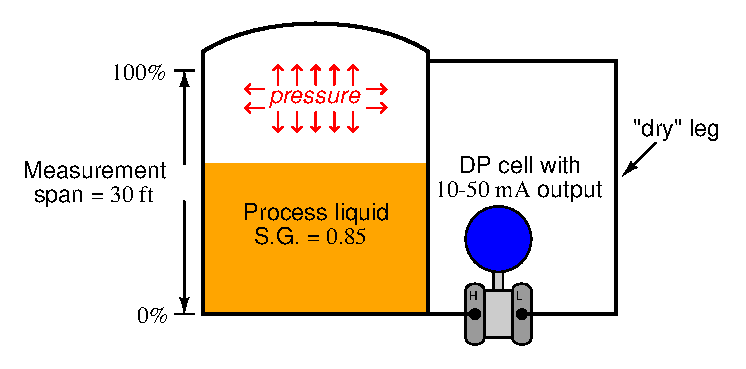
\includegraphics[width=15.5cm]{i00262x01.eps}$$

% No blank lines allowed between lines of an \halign structure!
% I use comments (%) instead, so that TeX doesn't choke.

$$\vbox{\offinterlineskip
\halign{\strut
\vrule \quad\hfil # \ \hfil & 
\vrule \quad\hfil # \ \hfil & 
\vrule \quad\hfil # \ \hfil \vrule \cr
\noalign{\hrule}
%
% First row
\% av spenn & $\Delta$P ("H$_{2}$O) & Utgang (mA) \cr
%
\noalign{\hrule}
%
% Another row
0 &  &  \cr
%
\noalign{\hrule}
%
% Another row
50 &  &  \cr
%
\noalign{\hrule}
%
% Another row
100 &  &  \cr
%
\noalign{\hrule}
} % End of \halign 
}$$ % End of \vbox

Anta nå at tanken varmes opp, og væsken i tanken avgir kondenserbare damper.  Disse kondenserer i low-side-røret til $\Delta$P-transmitteren, som er kjøligere enn lagertanken, slik at vi får et ``wet leg'' i stedet for ``dry leg''.  Med andre ord vil transmitteren nå ``se'' en konstant væskesøyle (SG = 0.85) på 30 fot koblet til ``low''-prosessen:

$$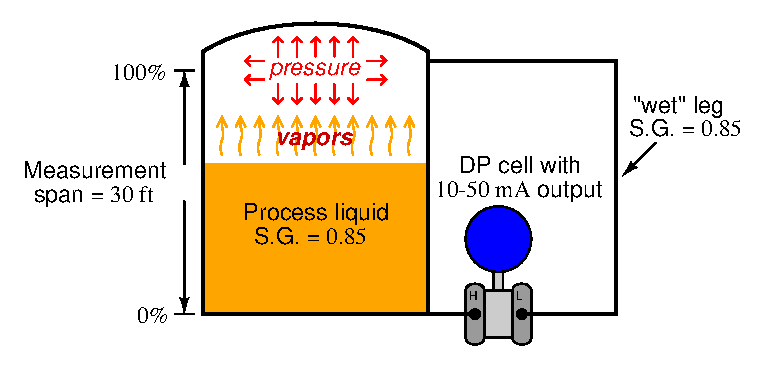
\includegraphics[width=15.5cm]{i00262x02.eps}$$

Beregn på nytt 0\%, 50\% og 100\% kalibreringspunkter for $\Delta$P-transmitteren med vått referanseben i stedet for tørt.

% No blank lines allowed between lines of an \halign structure!
% I use comments (%) instead, so that TeX doesn't choke.

$$\vbox{\offinterlineskip
\halign{\strut
\vrule \quad\hfil # \ \hfil & 
\vrule \quad\hfil # \ \hfil & 
\vrule \quad\hfil # \ \hfil \vrule \cr
\noalign{\hrule}
%
% First row
\% av spenn & $\Delta$P ("H$_{2}$O) & Utgang (mA) \cr
%
\noalign{\hrule}
%
% Another row
0 &  &  \cr
%
\noalign{\hrule}
%
% Another row
50 &  &  \cr
%
\noalign{\hrule}
%
% Another row
100 &  &  \cr
%
\noalign{\hrule}
} % End of \halign 
}$$ % End of \vbox

\underbar{file i00262}
%(END_QUESTION)





%(BEGIN_ANSWER)

{\bf Dry leg:}

% No blank lines allowed between lines of an \halign structure!
% I use comments (%) instead, so that TeX doesn't choke.

$$\vbox{\offinterlineskip
\halign{\strut
\vrule \quad\hfil # \ \hfil & 
\vrule \quad\hfil # \ \hfil & 
\vrule \quad\hfil # \ \hfil \vrule \cr
\noalign{\hrule}
%
% First row
\% av spenn & $\Delta$P ("H$_{2}$O) & Utgang (mA) \cr
%
\noalign{\hrule}
%
% Another row
0 & 0 & 10 \cr
%
\noalign{\hrule}
%
% Another row
50 & 153 & 30 \cr
%
\noalign{\hrule}
%
% Another row
100 & 306 & 50 \cr
%
\noalign{\hrule}
} % End of \halign 
}$$ % End of \vbox

\vskip 10pt

{\bf Wet leg:}

% No blank lines allowed between lines of an \halign structure!
% I use comments (%) instead, so that TeX doesn't choke.

$$\vbox{\offinterlineskip
\halign{\strut
\vrule \quad\hfil # \ \hfil & 
\vrule \quad\hfil # \ \hfil & 
\vrule \quad\hfil # \ \hfil \vrule \cr
\noalign{\hrule}
%
% First row
\% av spenn & $\Delta$P ("H$_{2}$O) & Utgang (mA) \cr
%
\noalign{\hrule}
%
% Another row
0 & -306 & 10 \cr
%
\noalign{\hrule}
%
% Another row
50 & -153 & 30 \cr
%
\noalign{\hrule}
%
% Another row
100 & 0 & 50 \cr
%
\noalign{\hrule}
} % End of \halign 
}$$ % End of \vbox

%(END_ANSWER)





%(BEGIN_NOTES)


%INDEX% Measurement, level: hydrostatic pressure (elevated zero)
%INDEX% Measurement, level: hydrostatic pressure (``wet'' reference leg)

%(END_NOTES)
